\documentclass{article}
\usepackage{hyperref}
\usepackage{graphicx}
\graphicspath{ {figures/} }

\begin{document}

\newcommand{\link}[2]{\textbf{\href{#1}{#2}}}

\title{Wargame: Red Dragon Internal Mechanics Manual}
\date{\today}
\author{Resident Mario}
\maketitle

\newpage
\tableofcontents
\newpage

\section{Introduction}

This document lays out the structure and internal mechanics of the units in RTS video game Wargame: Red Dragon (and thereof, of the entire Wargame series). Over the course of its release the series has garnered a sizable modding community, one which has done much great work tinkering with the game and exploring the boundaries it lays out. Much credit goes in particular to Enohka, whose \link{https://github.com/enohka/moddingSuite}{Wargame Modding Suite} makes studying and patching the game's files  easy and intuitive (or at least as easy and intuitive as modifying a game of this complexity can be).

This document was prepared and published in support of an initiative in the \link{https://github.com/ResidentMario/wargame-data}{extraction and datafication} of the 1,800+ units in Wargame: Red Dragon. In its attempt to summarize in detail all that is known about the game units' interals it has many precursors. Although there are other aspects to modding, unit creation and modification is easily the most heavily travelled and easiest aspect to modding the game, and it is the explicit focus of this text.

All numbers and counts in this guide refer to Wargame: Red Dragon circa late-2016, version 510049986.

\newpage

\section{Getting Started}

This guide is written from the perspective of the Wargame Modding Suite. If you have not done so already, download this wonderful tool.

When you open up the Modding Suite for the first time, it should be able to find a reference to your most recent copy of Wargame: Red Dragon. If it does not, or you want to switch versions, click on "Open" in the taskbar, then navigate to your game's copy of the data file you would like to open.

Wargame database files are backed up, with the structure and contents of each previous version of the game backed up in its own folder on disk. The practical reason for this additional use of space is that it enables the in-game replay viewer, which obviously relies on the gamestate being what it was at the time that the game took place. It does take up additional space, but the files are relatively small compared to the game's art and physics assets, and having the game's history also lets us explore what it looked like in the past (something most other games don't allow).

As a consequence of this organization, files related to various patch versions of the game are stored as subdirectories of a top-level data folder: \break \texttt{C:/Steam/steamapps/common/Wargame Red Dragon/Data/WARGAME/PC} on my disk. If you open this folder you will see a descending list of folders, each of which refering to a specific patch version of the game. The higher the number, the more recent the version. Naturally the highest number corresponds to the most recent version, and the lowest number to the first release version.

The most recent version as-of-writing is 510049986. Each version of the game will be a similar 9-digit string. The first two elements are the major version number, while the last five (last three in older versions) is the patch number.

Each patch is accompanied by a Eugen changelist in the forums, so to find out what changes were applied in which patches, search that number in their forums. The major content patches are described in \link{http://forums.eugensystems.com/viewtopic.php?f=155&t=57546}{series of forum posts}; go there to see them.

Every folder contains \texttt{NDF\_Win.dat}, which is the primary database file for that version of the game. Information internal to Wargame follow an ascending schema: information and assets introduced in the first version of the game which do not recieve any patches along the way (like almost all the art assets, for example) continue to live wherever they were first introduced, and do not get copied "up" the patch list. When Wargame initialized, the Loading Screen is actually the game working to link all of these changes up together to get a working schema of the current version of the game.

Within NDF\_Win, things are organized in terms of files of the "ndfbin" type. The most important of these is "everything.ndfbin", which contains nearly all easily modifiable attributes of the game. This file, decompiled by the Modding Suite, in turn consists of a couple hundred tables. These tables, or "modules", are linked to one another within a complex hierarchy.

The most important table, for our purposes, is TUniteAuSolDescriptor. This table is top-level object describing all of the purchasable and playable units in the game (as well as a variety of deprecated and occassional "special" ones):

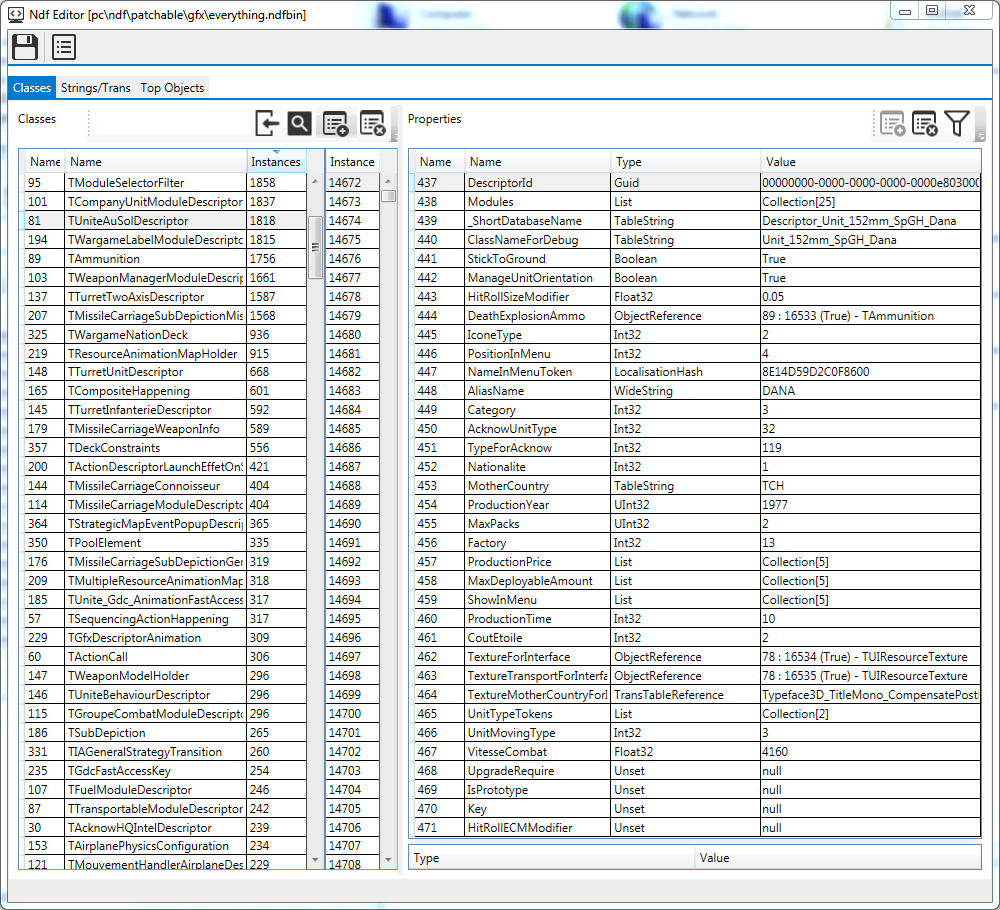
\includegraphics[width=0.8\textwidth]{screenshot_everything}


A sister table, TUniteDescriptor, describes both these units and additionally missiles, leading to a first, mildly amusing observation: missiles in the game are treated as their own units by the engine.

This table is our starting point.

Note that the first entry in this table is the 90-point Czech DANA artillery piece, which happens to, arbitrarily, have the lowest table ID in the game. This is followed by a Polish KUB-M anti-air unit, and then by a Russian Tunguska anit-air unit, as good a starting point as any other. 

\newpage

\section{TUniteAuSolDescriptor}

\subsection{DescriptorId}

This is a multi-part hex hash that is used internally by the engine. It is a unique key for the table. Don't touch it.

\subsection{\_ShortDatabaseName}

Prepended version of \_ClassNameForDebug.

\subsection{\_ClassNameForDebug}

An always-present non-localized unit name. Sometimes not entirely serious: for instance, Li Jian are given the moniker "Chinese Swords", while South Korean elite spec ops are "Black Berets". Not the name displayed in-game.

\subsection{StickToGround}

True if the unit is a ground unit, else null.

\subsection{ManageUnitOrientation}

Null for infantry units, True otherwise.

It is believed that this controls whether or not the unit can be given a position orientation command (Shift+Drag) in-game. 

\subsection{HitRollSizeModifier}

The effect that the size of the unit has on the chance-to-hit of other units firing at it. Larger-than-average units have a high HitRollSizeModifier, smaller-than-average ones have a low HitRollSizeModifier. This statistic is one of many calculations that factors into chance-to-hit.

The "Size" statistic in the armory screen is a direct translation of this variable. May be set to any float, but the values used in-game are:

\begin{center}
    \begin{tabular}{ | l | l | l | l | l |}
    \hline
	Value & Armory & Applies To & Example & Instances \\ \hline
	-0.2  &  Very Small & Scout helos & AH6C Little Bird  & 37\\
	-0.15 & Very Small & Infantry & Morskaya Pehota & 296 \\
	-0.1 & Very Small & Light helos & MI2URPG & 20 \\
	-0.05 & Small & Light vehicles & Scorpion Light Tank & 20\\
	null & Medium & Most things & BMP-1K & 958 \\
	0.05 & Big & Tanks, Heavy AA & M11P Abrams & 237\\
	0.1 & Very Big & Large helos & Mi-26 & 9\\	
    \hline
    \end{tabular}
\end{center}

\subsection{DeathExplosionAmmo}

A reference to a TAmmunition module which explodes in-place when this unit dies. This is a clever secondary use of TAmmunition, which is covered elsewhere in this guide.

At present time, units explode with one of just 11 animations. This includes null (e.g. no animation) which probably in error applies only to the Polish Star 266 supply truck.

\subsection{IconeType}

Unknown. Options are 1 (default), 2 (artillery and anti-ship missiles), and 3 (anti-air).

\subsection{PositionInMenu}

Does nothing.

\subsection{NameInMenuToken}

This localization hash controls the display name of the unit in the menu.

As previously mentioned, Wargame database files are backed up, with the structure and contents of each previous version of the game backed up in its own folder on disk. To get what this token corresponds to, we actually have to exit NDF\_Win.dat and load ZZ\_Win.dat instead (if this file is not present in your folder, check the immediately prior patch versions, one of them should have it). This file contains all of the text localization strings for the game. The \texttt{unites.dic} in particular contains all of the English-language menu texts, and if you for example look up our Dana's 8E14D59D2C0F8600 hash in this table you will find that it is, indeed, called the DANA in-game.

Thus you can change this yourself by editing this hash or by creating new ones and refering to them using the Modding Suite.

It needs to be noted that this piece of text corresponds to the name in the armory screen only. A second hash with the same name stored in the UnitType submodule, which we will get to later, controls the unit's name in-game.

\subsection{AliasName}

A better-formed name for the unit. Does nothing in-game. Not editable. Some are null.

\subsection{Category}

Unknown.

\subsection{AcknowUnitTpye}

Unknown.

\subsection{TypeForAcknow}

Unknown.

\subsection{Nationalite}

NATO units are null, PACT units are 1.

\subsection{MotherCountry}

An abbreviation for the country of origin of this unit.

\begin{center}
    \begin{tabular}{ | l | l |}
    \hline
	Value & Nation\\ \hline
	US & United States\\
	UK & United Kingdom\\
	FR & France\\
	RFA & West Germany\\
	CAN & Canada\\
	SWE & Sweden\\
	NOR & Norway\\
	DAN & Denmark\\
	ANZ & ANZAC\\
	JAP & Japan\\
	ROK & South Korea\\
	ISR & Israel\\
	HOL & The Netherlands\\
	URSS & Soviet Union\\
	RDA & East Germany\\
	TCH & Czechoslavakia\\
	POL & Poland\\
	CHI & China\\
	NK & North Korea\\
    \hline
    \end{tabular}
\end{center}

These are French acronyms, hence why URSS is "backwards".

\subsection{ProductionYear}

The year that the unit was produced. Note that this variable only controls the text; whether or not the unit is actually available in the unit-year categories for deck building (Cat A, Cat B, Cat C) is controlled elsewhere.

\subsection{MaxPacks}

The number of cards of this unit which are available for deck-building. Ranges from 1 (542 instances) or 2 (995 instances, the most common) up to 9 (16 instances, for certain transports).

\subsection{Factory}

Armory tab. Values are:

\begin{center}
    \begin{tabular}{ | l | l | l |}
    \hline
	Value & Tab & Count\\ \hline
	3 & Logistics & 177\\
	6 & Infantry & 233\\
	7 & Planes & 214\\
	8 & Vehicles & 335\\
	9 & Tanks & 196\\
	10 & Recon & 197\\
	11 & Helicopters & 142\\
	12 & Ships & 65\\
	13 & Support & 259\\
    \hline
    \end{tabular}
\end{center}

\subsection{ProductionPrice}

The in-game production price. This value isn't provided straight, but is instead embedded into a Collection of five integer elements. This may be because production price was at one point experimentally dependent on the veterancy of the unit, but this mechanic is not used in-game. Instead, the first value in this list is the actual price, and the remainder are all placeholder values of 15.

\subsection{MaxDeployableAmount}

A Collection of integers. The amount of copies of this unit deployable at each veterancy level, per card. 0 for veterancies this unit is not available at. Ordered Rookie to Elite.

\subsection{ShowInMenu}

A Collection of booleans which is always set to True for true units and always set to False for missiles.

\subsection{ProductionTime}

How long it takes, between an air unit being clicked on or a squad of land units being places on the map, for the unit to appear where it's expected. Airplanes have a ProductionTime of null (instantaneous), most units have a ProductionTime of 10, and helicopters have a ProductionTime of 5. This value is in seconds.

\subsection{CoutEtiole}

Means "Price Star" in French. A quickly-dropped mechanic in the first iteration of the series, Wargame: European Escalation, was that unit cards for your deck, besides the basic ones, would cost an in-game currency known as "stars" to unlock. This variable used to control this cost, and continues to exist today as a holdover. Seems to always be set to 1, 2, or 3, and doesn't do anything.

\subsection{TextureForInterface}

A reference to the texture resource for this object's deck display.

\subsection{TextureTransportForInterface}

Transport units can appear in the armory screen as seperate units, but most of the time they are viewed during deck building "behind" the units they are carrying, in which case this texture reference is called up and placed. Is set to null for non-transport units.

\subsection{TextureMotherCountryForInterface}

Controls which flag gets displayed in the corner of the card display.

\subsection{UnitTypeTokens}

A list of LocalizationHash instances which control which deck type the unit falls into. Valid inputs are:

\begin{center}
    \begin{tabular}{ | l | l |}
    \hline
	Kind & Hash\\ \hline
	Mechanized & 8BD43C9757360E00\\
	Armored & 5C76718B57360E00\\
	Marine & 23B8605ED9380000\\
	Airborne & 0BB7685ED9380000\\
	Motorized & 5E767965E3000000\\
	Support & DAD77965E3000000\\
    \hline
    \end{tabular}
\end{center}

\subsection{UnitMovingType}

Flags the unit movement type. Values are:

\begin{center}
    \begin{tabular}{ | l | l | l |}
    \hline
	Value & Kind & Count\\ \hline
	1 & Foot & 296\\
	2 & Wheeled, Supply Truck, Land-Only & 36\\
	3 & Wheeled, Non-Supply Truck, Land-Only & 215\\
	5 & Tracked, Land-Only & 445\\
	6 & Planes, Helicopters & 448\\
	7 & Wheeled, Amphibious & 121\\
	8 & Tracked, Amphibious & 225\\
	9 & Ship & 32\\
    \hline
    \end{tabular}
\end{center}

A unit's track style controls how it moves, and this field contains some important information on this subject.

Units moving on foot (1) move at the same speed on land everywhere, can move on steep slopes, and cannot enter water. 

Wheeled units in general (2, 3, 7) move at 150 kph on roads, regardless of off-road speed (specified in MouvementManager), and move at 33\% of their off-road speed in forests. Amphibious wheeled units (7) can additionally enter water, moving at a globally-set 50\% of their off-road speed when doing so. I do not know what the difference between (2) and (3) is.

Tracked units in general (5, 8) move at 110 kph on roads, regardless of off-road speed (specified in MouvementManager), and move at 50\% of their off-road speed in forests. Amphibious tracked units (8) can additionally enter water, moving at a globally-set 50\% of their off-road speed when doing so.

It should be noted that while 150 kph and 110 kph are global values, they are not controlled globally. There is instead a multiplier in another submodule, MouvementDescriptor, called RoadSpeedBonus, which is always set to exactly what it has to be set to to make this fact true. Amphibiousness, by contrast, is universial: if the unit can tread water, it will do so at half of its off-road speed, and as no other variables control this behavior this happens without exceptions.

\subsection{VitesseCombat}

According to the name, the speed of the unit when it is in combat (e.g. whenever the unit can see enemy units). It is surprising that this is a top-level variable and unknown whether or not this variable has any effect. The input is an unsigned int; for information on what the unit of measurement is, refer elsewhere in this guide.

\subsection{UpgradeRequired}

Contains a reference to another TUniteAuSolDescriptor. When this unit is pulled up in the armory, assuming you did all of the other categorization placements right, this unit will display after the linked unit in the horizontal list. If this is set to null, the unit will appear either on its own line or as the first unit in the horizontal list, if another unit references it itself.

Five is the maximum value, as no more are allowed to stack in the armory; any number higher will move the unit to its own line. It's also notable that when transport units are linked via UpgradeRequired, if one unit is made available as a transport for a unit all of its children are, too (for example: enabling Mi-8T for Gornostrelki also enables Mi-8TVs).

\subsection{IsPrototype}

Whether or not the unit is a prototypal unit. Null if it isn't, True if it is. Affects deck-building, as prototypal units can't be used in global decks.

\subsection{Key}

Unknown. Almost always null.

\subsection{HitRollECMModifier}

The unit's ECM level. This only applies to planes and ships with higher than 0\% ECM; all other units (including planes without ECM) have this value set to null.

\subsection{Modules}

A list of submodules attached to this unit:


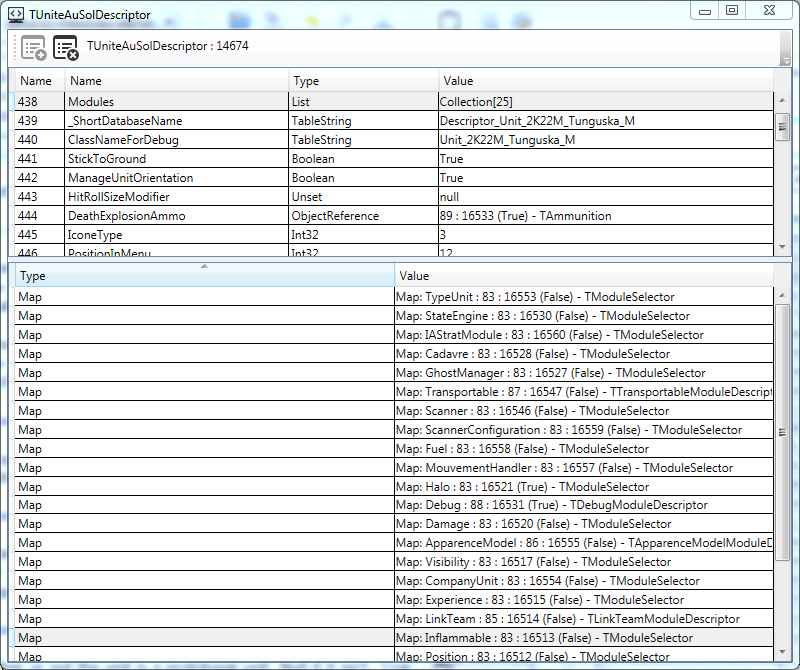
\includegraphics[width=0.8\textwidth]{screenshot_modules}

Each of these passes through a TModuleSelector to another table of some kind. We will now go through each of these in order of appearance.

\section{TTypeUnitModuleDescriptor}

\subsection{ControllerName}

Always TypeUnitController. Immutable.

\subsection{TypeUnitValue}

Unknown.

\subsection{TypeUnitHintToken}

Unknown.

\subsection{NameInMenuToken}

Just like its top-level NameInMenuToken, except that this copy of the hash controls what the unit's name is in-game, wheras the top-level one controls what it is in-menu. For more details see the UniteAuSol NameInMenuToken field.

\subsection{GenerateName}

Unknown. Always True.

\subsection{Filters}

This complex field is a Map containing four sets of things.

The first element is an in-game hover name which displays when a unit is hovered over by an enemy. An example value is "Anti-Air Vehicle".

The second element controls which of the year-based deck types the unit falls into (Cat A, Cat B, or Cat C). A dictionary for the values is:

\begin{center}
    \begin{tabular}{ | l | l | l |}
    \hline
	Value & Kind\\ \hline
41E22D4DD9380000 & 1980 and less\\
46E22D4DD9380000 & 1981 to 1985\\
81E22D4DD9380000 & 1986 and later\\
    \hline
    \end{tabular}
\end{center}

Note that it is this field, not the YearProduced top-level variable (which only controls an element of the card display), which controls which year-limited deck categories the unit is available in.

The third element is a set of the deck types that the unit appears in. But wait, you may ask, doesn't the top-level UnitTypeTokens already do that? It turns out that to make things work you have to properly set both that value and this one. Again, here's a list of valid hashes:

\begin{center}
    \begin{tabular}{ | l | l |}
    \hline
	Kind & Hash\\ \hline
	Mechanized & 8BD43C9757360E00\\
	Armored & 5C76718B57360E00\\
	Marine & 23B8605ED9380000\\
	Airborne & 0BB7685ED9380000\\
	Motorized & 5E767965E3000000\\
	Support & DAD77965E3000000\\
    \hline
    \end{tabular}
\end{center}

The fourth element is a set of hashes for miscellaneous filters that the unit falls under in the armoy. So for example if you want a unit to fall the "Cavalry Tank" filter there, you would need to set the appropriate hash here. The values for these hashes in particular are located in the interface\_ingame.dic file inside ZZ\_Win.dat.

\subsection{MotherCountry}

A copy of the top-level attribute.

\subsection{UnitInfoJaugeType}

Unknown.

\subsection{Training}

Unknown. Usually, maybe always null.

\subsection{CIWS}

The CIWS statistic, as displayed in the armory, carried by a naval unit. Set to null for non-naval units and for naval units without CIWS. This is a localization hash; to set it to a particular value, use one of the following:

\begin{center}
    \begin{tabular}{ | l | l |}
    \hline
	Kind & Hash\\ \hline
	Exceptional & 4F233E0000000000\\
	Very Good & 4E96452000000000\\
	Good & 4E96450000000000\\
	Medium & D672711906000000\\
	Bad & CEC2000000000000\\
	None & null\\
    \hline
    \end{tabular}
\end{center}

Changing this value does NOT change a ship's CIWS, it only changes the quality of CIWS reported on the card in-game. In other words, this only controls a text display element.

\subsection{Sailing}

The ship's sailing type. This is similarly a LocalizationHash controlling a text display, not the real value (which is in MouvementControl). Values are:

\begin{center}
    \begin{tabular}{ | l | l |}
    \hline
	Kind & Hash\\ \hline
	Deep Sea & CBD32D65B4780000\\
	Coastal & CBD33165B4780000\\
	Riverine & CBD33565B4780000\\
	None & null\\
    \hline
    \end{tabular}
\end{center}

\section{TDebugModuleDescriptor}

There is nothing interesting here.

\section{TStateEngineModuleDescriptor}

There is nothing interesting here.

\section{TFlagsModuleDesciptor}

Uknown.

\section{TCriticalEffectModuleDesciptor}

A reference to one of a small number of tables which control the critical effects a unit may be subjected to that occur due to fire from enemy units (critical effects affecting movement are in a different module, Mouvement). We will omit further details, as the resultant tables are various, singular, and pretty easy to parse.

\section{TTargetCoordinatorModuleDescriptor}

There is nothing interesting here.

\section{TPositionModuleDescriptor}

\subsection{ControllerName}

Not interesting.

\subsection{InGeoDb}

Unknown.

\subsection{ClampInWorld}

Unknown.

\subsection{GfxDescriptorPorteur}

Links to a module containing information of interest to the physics engine, which shouldn't be messed with.

\subsection{Radius}

Unknown.

\subsection{AddToHexagonMap}

Unknown.

\subsection{PorteurMustBeVisible}

Unknown.

\subsection{RelativeScanningPosition}

Unknown.

\subsection{CameraFollower}

Links to a TGfxDescriptorCameraFollower object that sets variables for the camera, meant for focus-watching a plane, land unit, ship, or helicopter.

\subsection{MustAllowZoneIndice}

Unknown.

\subsection{LowAltitudeFlyingAltitude}

If the unit is a helo, the altitude that the helo flies at by default.

\subsection{NearGroundFlyingAltitude}

If the unit is a helo, the altitude the helo goes to when told to descend (which helps with stealth, but is barely ever used anymore).

\subsection{ClampOutMap}

Unknown, always null.

\subsection{HasNearlyNullBBox}

Unknown, always null.

\subsection{\_ShortDatabaseName}

Useless, always null.

\section{TInfammableModuleDescriptor}

There is nothing interesting here.

\section{TLinkTeamModuleDescriptor}

There is nothing interesting here.

\section{TModernWarfareExperienceManagerDescriptor}

\subsection{ControllerName}

Disinteresting.

\subsection{CanWinExperience}

There are only two possible table references: one with CanWinExperience set to null, which is applied to supply units and units without weapons, and one with CanWinExperience set to True, for everything else.

\subsection{ExperienceGainBySecond}

Always set to 0.1.

\subsection{KillExperienceBonus}

Always set to 2.5

\section{TIAStratModule}

This module contains a few hard-coded numerical references which are used for internal AI orchestration.

\section{TModernWarfareCadavreModuleDescriptor}

This module is buried in the logic section of the CadavreController top-level module object. It contains a number of interesting variables, all controlling what happens when a unit dies: how long it sticks around afterwards, how quickly it fades, whether or not it exploded on death (if it does, it uses the DeathExplosionAmmo top-level object), and a bunch of flags:

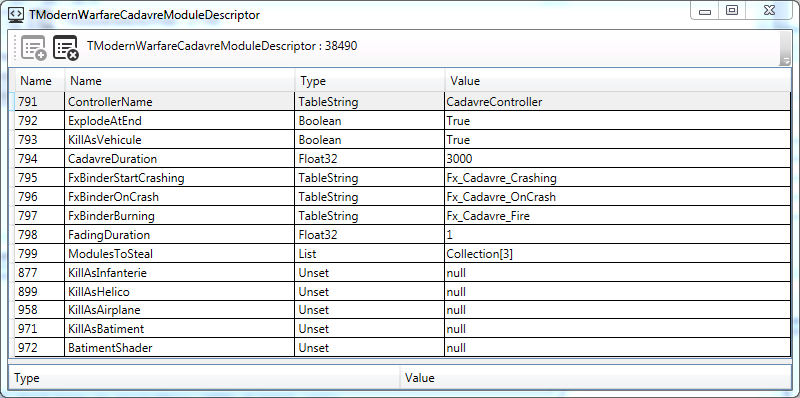
\includegraphics[width=0.8\textwidth]{screenshot_cadavre}

We will omit examining it in detail.

\section{TTurretSkeletonModuleDescriptor}

Contains a pointer to the unit's primary mesh.

\section{TMissileCarriageModuleDescriptor}

Contains pointers to art resources constituting missile carriages, which control all of the art involved in units having and then not having certain visible weapon elements on-body. So for example, a F-15D Eagle with its bombs would look different from an F-15D Eagle without its bombs, obviously. That's controlled here.

We will omit further details, except to say that the difficulties of working with this module make modding planes and helicopters (some of which have this module, some of which haven't) challenging.

\section{TCommandManagerModuleDescriptor}

When this module is set up properly, the unit is treated as a command unit in-game.

\section{TGhostManagerModuleDescriptor}

This module controls things related to what happens when a unit is spotted, but not identified: what you see when something is shaded in black. 

\section{TScannerModuleDescriptor}

This module is only present if the unit has special vision privileges. It contains a TModernWarfareVisibilityRollRule as a subtable, which in turn contains TModernWarfareVisibilityRollRuleDescriptor and TModernWarfareDistanceMultiplierRollRuleDescriptor dependencies.

A relatively small number of tables of the latter two types ultimately control large swatches of unit vision ranges, so you might find that e.g. tweaking one Very Good recon unit's table's vision range up will turn up vision for ALL Very Good recon units, and other similar shenanigans.

Types of vision controlled by this module are Air, Sea, and Land.

This module only contains multipliers. Base vision values are set by the module below.

\section{TScannerConfigurationDescriptor}

This module, if present, controls the base vision values for units granted above-normal vision. All of the base values come from here, but interact with values in TScannerModuleDescriptor above. If one of these two modules is present, both are, as they are dependent on one another.

\subsection{ControllerName}

Always ScannerConfigurationController. Immutable.

\subsection{UnitType}

A reference to the domain of the unit in question itself. UnitType 1 refers to ground, UnitType 4 refers to planes, and UnitType 6 refers to ships.

\subsection{DetectionTBA}

Maximum range at which you can see an unidentified helicopter.

\subsection{PorteeVision}

Maximum range at which you can see an unidentified ground unit.

\subsection{OpticalStrength}

Optical strength against ground units, used to determine whether a unit can see enemy units in cover.

\subsection{OpticalStrengthAltitude}

Optical strength against aircraft (including helicopters).

\subsection{SpecializedOpticalStrengths}

This is a Collection of float pair mapping; each of the maps binds a UnitType and then the range at which they can be detected. UnitType 4 refers to planes, while UnitType 6 refers to ships, and UnitType 1 refers to Land. The value Optican strengths against 

\subsection{SpecializedDetections}

Maximum range at which you can see an unidentified unit. This is a Collection of float pair mapping; each of the maps binds a UnitType and then the range at which they can be detected. UnitType 4 refers to planes, while UnitType 6 refers to ships, and UnitType 1 refers to Land.

\subsection{PorteVisionTBA}

Maximum spotting range for helicopters. This attribute is only populated for helicopters, in which case it controls helicopter-to-helicopter sighting. It is otherwise null.

\subsection{OpticanStrengthAntiradar}

Maximum anti-radar spotting range. Only populated for anti-radar units; null otherwise.

\subsection{\_ShortDatabaseName}

Same as the top-level parameter, but this seems to always be null.

\section{TFuelModuleDescriptor}

\subsection{ControllerName}

Uninteresting.

\subsection{FuelCapacity}

The number of units of fuel that this unit can stockpile.

\subsection{FuelMoveDuration}

Autonomy in seconds. Appears to b the same as the T.O.T statistic displayed in the Armory.

\section{TMovementHandlerLandVehicleDescriptor}

This module will only be present if the vehicle in question is, indeed, a land unit.

\subsection{ControllerName}

Uninteresting.

\subsection{Maxspeed}

The unit's max speed, in engine distance units (see the next major section for unit explanations).

\subsection{UnitMovingType}

The same as that set in TUnitMouvementDescriptor.

\subsection{SpeedBonusOnRoad}

A multiplier on the unit's base speed. Always set to whatever it needs to be set to to give the unit 110kph tracked speed or 150kph wheeled speed, meaning that these are constants but must be set on the local level!

\subsection{TempsDemiTour}

The amount of time, in seconds, it takes for a unit to make a half-turn (the translation is literal). If you tell a unit to move in a direction directly opposite to its current orientation, it will do a reverse-accelerate V-turn to the side, and this variable controls how long this takes.

Presumably this value also controls how long it takes to make turns that are less than 360 degrees, but still significant. The cutoff value at which a unit starts to make a reverse turn, instead of just turning in place, is unknown.

\subsection{MaxAcceleration}

The acceleration the unit applies when it is speeding up.

\subsection{MaxDeceleration}

How hard to breaks hit. Tends to be twice MaxAcceleration for tracked and wheeled land units.

\subsection{VehicleSubType}

Unknown, often null.

\subsection{CriticalEffectModule}

A module pointer whose contents is a TCriticalEffectModuleDescriptor describing what happens when this units is hit with a critical. Unfortunately it ultimately points to hashes, not to any descriptions of the effects of the criticals themselves...

\subsection{TerrainsToIgnoreMask}

This is set to certain magic values for ship units which are allowed and not allowed to enter different water depths: 16 if it can enter all waters, 24 if it's a coaster, and 26 if it's a bluewater ship.

Otherwise null.

\section{TMouvementHandlerHelicopterDescriptor}

\subsection{ControllerName}

Uninteresting.

\subsection{Maxspeed}

The unit's max speed, in engine distance units (the meaning of which is covered elsewhere).

\subsection{MaxAcceleration}

The acceleration the unit applies when it is speeding up.

\subsection{MaxDeceleration}

How hard the breaks hit.

\subsection{UnitMovingType}

The same as that set in TUnitMouvementDescriptor. Here this will always be 6, for air.

\subsection{CyclicManoeuvrability}

Controls movement.

\subsection{GFactorLimit}

Controls movement.

\subsection{LateralSpeed}

Controls movement.

\subsection{Mass}

Controls movement.

\subsection{MaxInclination}

Controls movement.

\subsection{RotorArea}

Controls movement.

\subsection{TorqueManoeuvrability}

Controls movement.

\subsection{UpwardsSpeed}

Controls movement.

\subsection{CriticalEffectsModule}

A module pointer whose contents is a TCriticalEffectModuleDescriptor describing what happens when this units is hit with a critical. Unfortunately it ultimately points to hashes, not to any descriptions of the effects of the criticals themselves...

\subsection{TempsDemiTour}

The amount of time, in seconds, it takes for a unit to make a half-turn (the translation is literal). For helicopters this requires a dive to the left. It's uncertain whether or not this variable is still used for anything.

\section{TMouvementHandlerAirplaneDescriptor}

\subsection{Maxspeed}

Maximum speed this unit can go at. Since airplanes fly at a constant speed, this is also the only speed.

\subsection{UnitMovingType}

Always 6, for air (other values are 4 for sea and 1 for land).

\subsection{FlyingAltitude}

The height the plane prefers to fly at. Notably, all planes spawn at the same height then ascend or descend to their prefered height.

\subsection{MinimalAltitude}

Below which the plane will not dip. Will cause it to break off from certain attacks at certain heights.

\subsection{PhysicsConfiguration}

A reference to a TAirplanePhysicsConfiguration module, which controls the plane's various movement parameters.

\subsection{CriticalEffectsModule}

A module pointer whose contents is a TCriticalEffectModuleDescriptor describing what happens when this units is hit with a critical. Unfortunately it ultimately points to hashes, not to any descriptions of the effects of the criticals themselves...

\subsection{GunMuzzleSpeed}

Unknown. Always 300000.

\subsection{LandingGearOutPhysicalPropertyName}

Unknown. Always "InShowRoom".

\subsection{LandingGearSubDescriptionName}

Unknown. Always "Landing Gear".

\subsection{FrontLandingGearMeshNodeName}

Unknown. Always "Train\_Avant".

\subsection{BackLandingGearMeshNodeName}

Unknown. Always "Train\_Arriere".

\section{THaloModuleDescriptor}

Does a bunch of things which control the circle that gets drawn when a unit is selected.

\section{TGroupeCombatModuleDescriptor}

This module, which is only attached to infantry units. This table has a submodule, TUniteBehaviorDescriptor, which has a large number of variables controlling the unique aspects of infantry combat stats in the game.

Amongst the various TUniteBehaviorDescriptor tables, all of the variables contained therein are the same (making them globals, essentially) except for two: NbSoldatInGroupeCombat, which controls the number of men to the squad, and AnimationFastAccessor, whose purpose is unknown.

\section{TTransportableModuleDescriptor}

This module, which is only attached to infantry units, controls what transports are available to an infantry unit.

\subsection{ControllerName}

Not interesting.

\subsection{Categories}

Always a list with two elements: "infantrie" and "barge".

\subsection{SuppressDamageRatioIfTransporterKilled}

This float controls what percentage of the unit's total suppression cealing (which is 800 for all units) the unit will take in suppression damage if it is on a transport, the transport is destroyed, and the unit survives.

As such it contains direct references to other transporter units' TUniteAuSolDescriptor instances.

\subsection{TransportListAvailableForSpawn}

This contains a Collection of references to one or more transporter units' TUniteAuSolDescriptor instances. Those units become available to this unit as an on-card transport.

Note that, due to the previously described mechanics of the UpgradeRequired top-level variable, a reference in this table to a transporter unit with an upgrade path will cause all of those other units to also become available. So the exactly list of transporters for this unit may be longer than it appears to be from this list alone!

\subsection{TransportedTexture}

Unknown. Transported units have no texture, no?

\section{TModuleModernWarfareSupplyDescriptor}

\subsection{ControllerName}

Uninteresting.

\subsection{SupplyCapacity}

Units of supply (liters) this unit carries.

\subsection{DeploymentDuration}

How long after a unit has stopped before it begins to provide supply, in seconds. Always 0.2 seconds currently, except for FOBs, which have this value set to null.

\subsection{WithdrawalDuration}

How long after a unit is ordered to start moving before it stops providing supplies and starts moving. Currently always 0.2 seconds currently, except for FOBs, which have this value set to null.

\subsection{SupplyPriority}

It is possible for supply units to supply other supply units; for example a common tactic is to shorten the supply chain trip length by buying a Mi-26, dropping it halfway between the FOB and the battlefield, and running ammo trucks between the helo and the front line. The lower this number the lower in this stack this unit is, and the greater the number of other supply units this supply unit could itself draw from. Generally 1-to-1 with total supply onboard: the bigger the capacity, the lower the SupplyPriority.

\subsection{SupplyDescriptor}

Links to another module, an instance of TModernWarfareSupplyDescriptor, which contains the variables used for calculating supply cost and supply per second. There are only two instances of TModernWarfareSupplyDescriptor, one for FOBs and one for all other supply units. The latter includes the following essentially-globals:

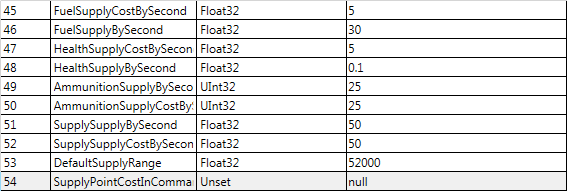
\includegraphics[width=0.8\textwidth]{screenshot_supply}

The former:

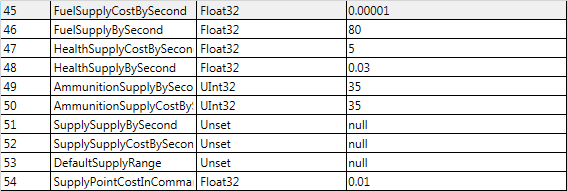
\includegraphics[width=0.8\textwidth]{screenshot_supply_fob}

\section{TWeaponManagerDescriptor}

WRITE THIS UP.

\section{TModernWarfareDamageModuleDescriptor}

WRITE THIS UP.

\section{TAppearanceModelDescriptor}

Controller for things related to the unit's appearance.

\section{TVisibilityModuleDescriptor}

\subsection{ControllerName}

Uninteresting.

\subsection{UnitStealthBonus}

A multiplier applied to the unit's visibility, and the only interesting contents of this module. The multipliers are:

\begin{center}
    \begin{tabular}{ | l | l | l | l |}
    \hline
	Value & Stealth & Examples & Counts\\ \hline
	0.1 & Bad & Hatsuyiki & 1\\
	0.3 & Bad & Luda & 1\\
	0.4 & Bad & Oliver Hazard Perry & 1\\
	0.5 & Bad & Jianghu III & 3\\
	0.6 & Bad & Nanushka III & 4\\
	0.7 & Bad & Donghae & 5\\
	0.8 & Bad & Chamsuri & 4\\
	0.9 & Bad & Shmel & 2\\
	1 & Poor & AMX-30B & 1349\\
	1.2 & Medium & Komar & 1\\
	1.25 & Poor (!) & MiG-29S & 1\\
	1.5 & Medium & VLB Minstral Recon & 139\\
	1.75 & Good & PAH-2 Tiger & 4\\
	2 & Good & US Marines & 200\\
	2.5 & Very Good & Spetsnaz GRU & 91\\
	3 & Exceptional & Spetsnaz VMF, Nighthawk & 7\\
    \hline
    \end{tabular}
\end{center}

\subsection{\_ShortDatabaseName}

The same as that set in the top-level object, but seemingly always null.

\section{TCompanyUnitDescriptor}

Companies are what the game terms sets of units ranging in size from 1 (lone) to 4 (max size; helicopters can only be grouped in 2s and planes and boats in 1s). This module contains a bunch of elements which define the logic of giving orders to a company of units, as well as the number limiting how many of the unit stack.

\end{document}